\section{Dynamik}
		
	\subsection{Newtonsche Gesetze}
		Gesetze, welche Bewegungen beschreiben.

		\subsubsection{Erstes Newtonsches Gesetz: Trägheitsgesetz}
			Ein Körper verharrt in seine Zustand (Ruhe, gleichförmige geradlinige Bewegung), wenn er nicht durch eine Kraft gezwungen wird, seinen Zustand zu ändern. \\
			\\
			Die \textbf{Trägheit} eines Körpers hängt von seiner (Trägheits-) Masse ab.
			
		\subsubsection{Zweites Newtonsches Gesetz: Aktionsgesetz}	
			\begin{minipage}{0.2\linewidth}
				$\boxed {\vec{F} = m \cdot \vec{a} }$
			\end{minipage}
			\hfill
			\begin{minipage}{0.75\linewidth}
				\begin{tabular}{c l c}
					$\vec{F}$ & Kraft & $[F] = \mathrm{\frac{kg \cdot m}{s^2}  = N}$ \\
					$m$ & (Trägheits-) Masse & $[m] = \mathrm{kg}$ \\	
					$\vec{a}$ &  Beschleunigung & $[a] = \mathrm{\frac{m}{s^2}}$ \\
					\\
				\end{tabular}
			\end{minipage}
				
			$\Rightarrow$ Anwendung erfolgt meist komponentenweise!
				
		\subsubsection{Drittes Newtonsches Gesetz: Wechselwirkungsgesetz}
			
		Wirkt ein Körper A auf einen Körper B mit der Kraft $\vec{F}_{AB}$, so wirkt der Körper B auf A mit der Kraft $\vec{F}_{BA} = - \vec{F}_{AB}$ \\

\vfill\null
\columnbreak	

	\subsection{Reibungskräfte}

		$$ \boxed{ \text{Haftreibung:} \quad  \vec{F}_{R,max} = \mu_H \cdot \vec{F}_N } $$ 
		
		$$ \boxed{ \text{Gleitreibung:} \quad \vec{F}_{Gleit} \approx \mu_G \cdot \vec{F}_N } $$ 
		
		$$ \boxed{ \text{Rollreibung:} \quad \vec{F}_{Roll} \approx \mu_R \cdot \vec{F}_N } $$ \\
		
		\begin{tabular}{c l c}
			$\vec{F}_R$ & Reibungskraft & $[\vec{F}_R] = \mathrm{N}$ \\
			$\vec{F}_{R,max}$ & Haftreibungskraft & $[\vec{F}_{R,max}] = \mathrm{N}$ \\
			$\vec{F}_{Gleit}$ & Gleitreibungskraft & $[\vec{F}_{Gleit}] = \mathrm{N}$ \\
		\end{tabular}

	\subsection{Rollreibungslänge $e$ (Drehmoment)}

		\begin{minipage}{0.48\linewidth}
			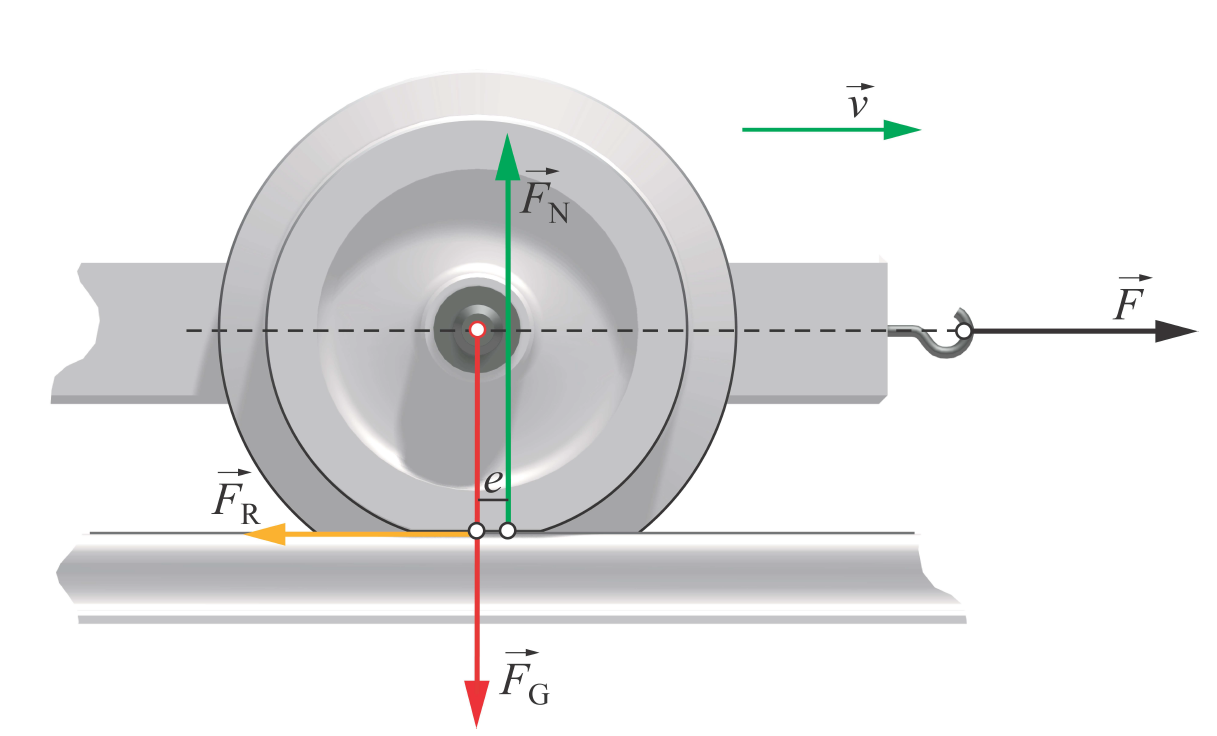
\includegraphics[width=0.8\linewidth]{Bilder/rollreibung_1} \\
		\end{minipage}
		\hfill
		\begin{minipage}{0.48\linewidth}
			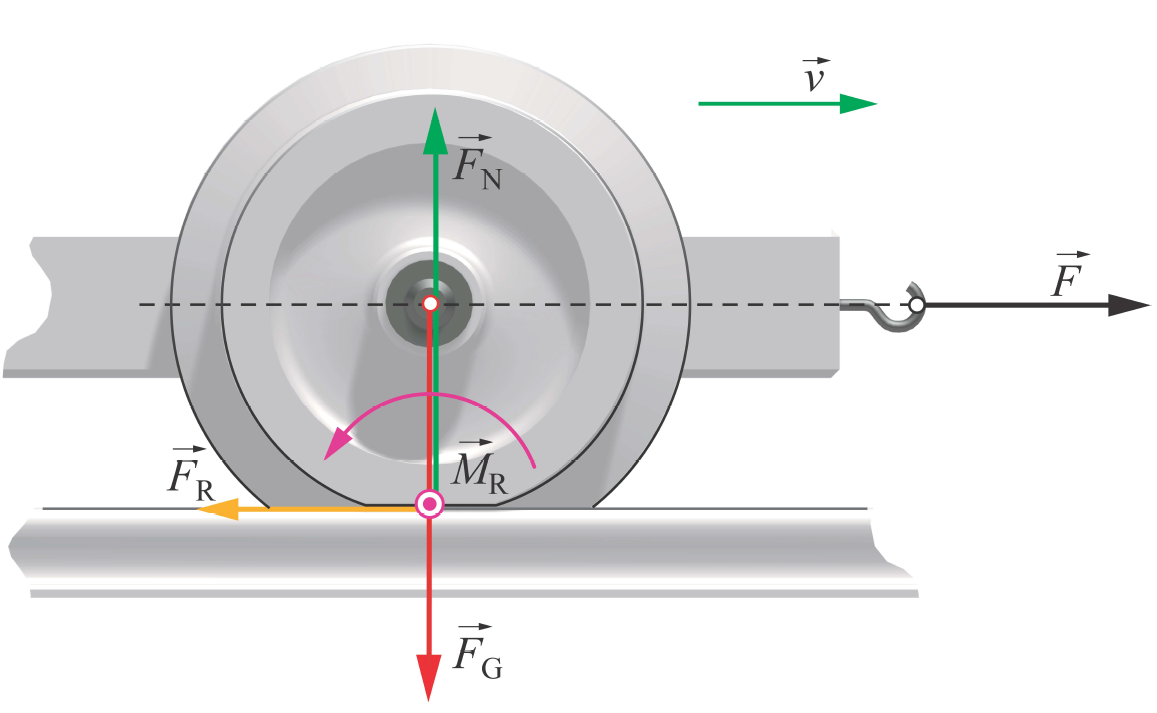
\includegraphics[width=0.8\linewidth]{Bilder/rollreibung_2} \\
		\end{minipage}
		
		$$ \boxed{ e = \frac{r \cdot F}{F_N} = \frac{r \cdot F_R}{F_N} =  \frac{r \cdot \mu_R \cdot F_R}{F_N} = \mu_R \cdot r }$$ 
		
		$$ \boxed{ M_R = e \cdot F_N = \mu_R \cdot r \cdot F_N = r \cdot F_R = r \cdot F} $$ \\

		\begin{tabular}{c l c}
			$e$ & Rollreibungslänge & $[e] = \mathrm{m}$ \\
			$r$ & Radius des Rades & $[r] = \mathrm{m}$ \\
			$F_R$ & Rollreibungskraft & $[F_R] = \mathrm{N}$ \\
			$F_N$ & Normalkraft & $[F_N] = \mathrm{N}$ \\
			$\mu_R$ & Rollreibungskoeffizient & $[\mu_R] = 1$ \\
			$M_R$ & Rollreibungsmoment & $[M_R] = \mathrm{Nm}$ \\
		\end{tabular}

	\subsection{Angetriebenes Rad}
	
		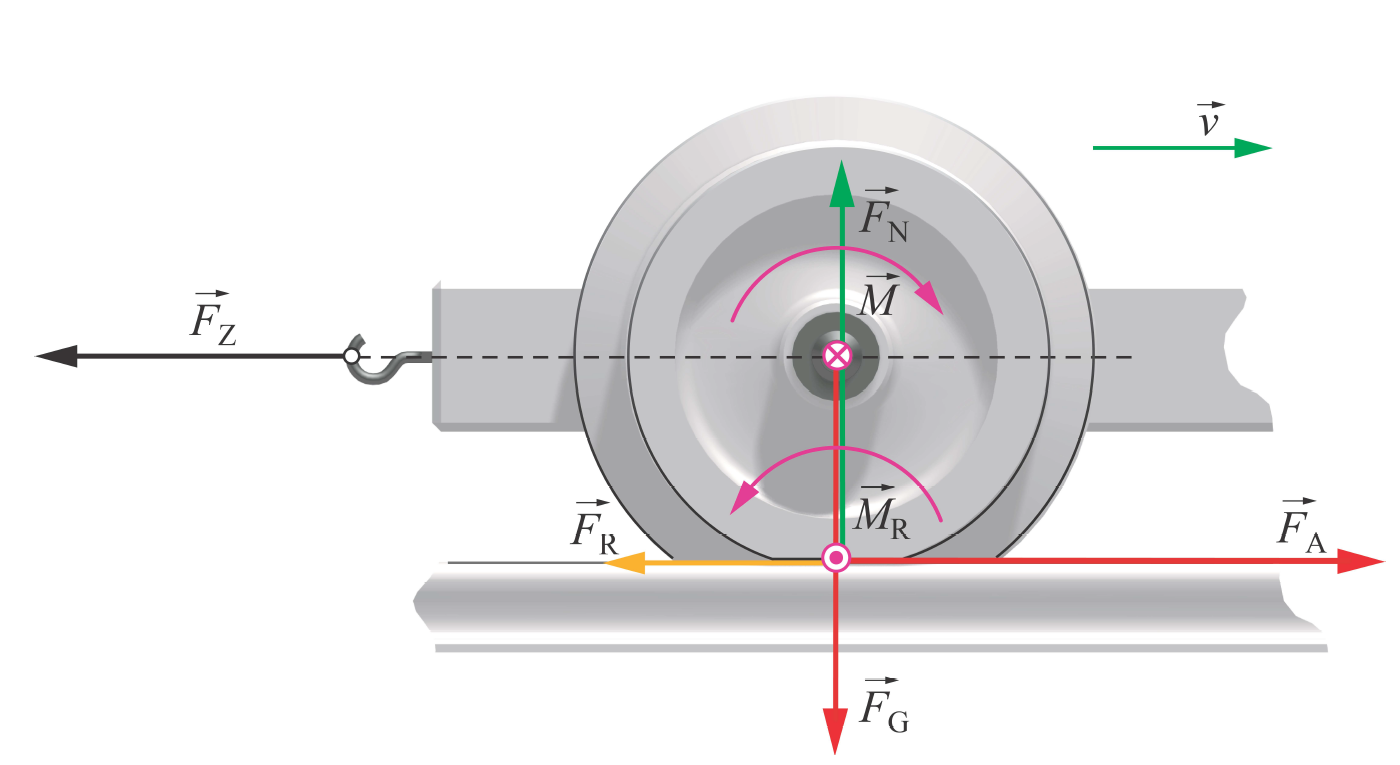
\includegraphics[width=0.8\linewidth]{Bilder/antriebsrad} \\
		\\

		\begin{tabular}{c l c}
			$\vec{F_Z}$ & Zugkraft & $[F_Z] = \mathrm{N}$ \\
			$\vec{F_N}$ & Normalkraft & $[F_N] = \mathrm{N}$ \\
			$\vec{F_R}$ & Rollreibungskraft & $[F_R] = \mathrm{N}$ \\
			$\vec{F_A}$ & Haftreibungskraft & $[F_A] = \mathrm{N}$ \\
		\end{tabular}

		\subsubsection{Hinweise zu Reibung an Rädern}
		
			\begin{tabular}{ll}
				$\bullet$ & Jedes Rad weist Rollreibung auf \\
				$\bullet$ & Zusätzlich zur Rollreibung weist ein angetriebenes Rad \\
				          & eine Haftreibung auf \\
			\end{tabular}

	\subsection{Arbeit und Energie}
	
		\subsubsection{Arbeit}
		
			Wird der Angriffspunkt einer Kraft $\vec{F}$ um die Strecke $d \vec{s}$ verschoben so leistet die Kraft die Arbeit $W$ 
			
			$$ \boxed{ W_{AB} =  \int \limits_A^B d \, W =  \int \limits_A^B \vec{F} \bullet d \, \vec{s} \qquad \text{(Skalarprodukt)} }$$ \\
			
			Wenn die projizierte Kraft konstant ist: $\boxed{ W = F \bullet s_{AB} }$ \\
			\\
			\begin{tabular}{c l c}
				$W$ & Arbeit & $[W] = \mathrm{N \cdot m = J}$ \\
				$F$ & Kraft & $[F] = \mathrm{N}$ \\
				$s$ & Weg & $[s] = \mathrm{m}$ \\
			\end{tabular}

		\subsubsection{Potentielle Energie $W_{pot}$}
			Beim Anheben eines Körpers gewinnt der Körper an potentieller Energie (Lageenergie) 
			
			$$ \boxed{ W_{pot} = m \cdot g \cdot h}$$
			\\
			\begin{tabular}{c l c}
				$W_{pot}$ & Potentielle Energie & $[W] = \mathrm{N \cdot m = J}$ \\
				$m$ & Masse des Körpers & $[m] = \mathrm{kg}$ \\
				$g$ & Erdbeschleunigung & $[g] = \mathrm{\frac{m}{s^2}}$ \\
				$h$ & Höhe der Körpers & $[h] = \mathrm{m}$ \\
				\\
			\end{tabular}
			
			\textbf{Beispiel: Spannen einer Feder} \\
				\\  
				Federkraft als Funktion der Auslenkung x \qquad $F = -k \cdot x$ \\
				\\
				$$ \boxed{ W_{pot} = \int \limits_0^{x_0}  - \vec{F} \bullet d \vec{x} = \int \limits_0^{x_0}  k \cdot x \, dx = \frac{1}{2} \, k \cdot x_0^2} $$ \\
				
			\begin{tabular}{c l c}
				$W_{pot}$ & Potentielle Energie & $[W] = \mathrm{N \cdot m = J}$ \\
				$F$ & Federkraft & $[F] = \mathrm{N} $ \\
				$k$ & Federkonstante & $[k] = \mathrm{\frac{N}{m}}$ \\
				$x_0$ & Auslenkung der Feder & $[x_0] = \mathrm{m}$ \\
			\end{tabular}

		\subsubsection{Kinetische Energie $W_{kin}$}
		
			$$ \boxed{ \normalsize{ W_{kin} = \int \limits_A^B \vec{F} \bullet d \, \vec{s} =  F \bullet s_{AB} = m \, a \cdot \frac{a}{2} t^2 = m \frac{a^2 \cdot t^2}{2} = \frac{1}{2} m \cdot v^2} }$$
			
			\begin{tabular}{c l c}
				$W_{kin}$ & Kinetische Energie & $[W] = \mathrm{N \cdot m = J}$ \\
				$F$ & Kraft & $[F] = \mathrm{N} $ \\
				$s$ & Wegstück (Kinematik) & $[s] = \mathrm{m}$ \\
				$m$ & Masse des Körpers & $[m] = \mathrm{kg}$ \\
				$a$ & Beschleunigung (Kinematik) & $[a] = \mathrm{\frac{m}{s^2}}$ \\
				$v$ & Geschwindigkeit (Kinematik) & $[v] = \mathrm{\frac{m}{s}}$ \\
			\end{tabular}

	\subsection{Energieerhaltung (in abgeschlossenen Systemen)}
	
		Die Gesamtenergie eines \underline{abgeschlossenen Systems} ist unveränderlich! \\
		\\
		\textbf{abgeschlossen: Es wird keine Masse hinzugefügt/entfernt und es wirken keine äusseren Kräfte!} \\
			\\	
			$$ \boxed{ W = \underbrace{m \cdot g \cdot h}_{\substack{\text{pot. Energie}}} =  m \cdot g \cdot \underbrace{ \frac{1}{2} \, g \cdot t^2}_{\substack{\text{h(t)}}}  = \underbrace{ \frac{1}{2} m \cdot v^2 }_{\substack{\text{kin. Energie}}} } $$ \\
			\\
			Für \underline{nicht abgeschlossene Systeme} kann eine Bilanzrechnung aufgestellt werden: \\
			Die Energiezunahme im Gesamtsystem entspricht der von aussen zugeführten Energie. \\
			Die Energieabnahme im Gesamtsystem entspricht der von aussen entzogenen Energie. \\

		\subsubsection{Energiesatz der Mechanik} 
			$$ \boxed{ E_{pot} + E_{kin} = E_{tot} = \text{const} } \qquad \text{(gilt zu jedem Zeitpunkt)} $$

	\subsection{Leistung und Wirkungsgrad}
	
		\subsubsection{Leistung}
		
			$$ \boxed{ P = \frac{\Delta W}{\Delta t} = \frac{\vec{F} \bullet \Delta \vec{s}}{\Delta t} = \vec{F} \frac{\Delta \vec{s}}{\Delta t} = \vec{F} \bullet \vec{v} } $$ 
			
			
			\begin{tabular}{c l c}
				$P$ & Leistung & $[P] = \mathrm{W = \frac{J}{s}}$ \\
				$\Delta W$ & geleistete Arbeit & $[W] = \mathrm{J}$ \\
				$\Delta t$ & verstrichene Zeit & $[t] = \mathrm{s}$ \\
				$F$ & Kraft & $[F] = \mathrm{N}$ \\
				$\Delta s$ & Wegstück & $[s] = \mathrm{m}$ \\
				\\
			\end{tabular}
			
			\textbf{Pferdestärken} \\
				\\
				$1 \; \mathrm{PS} = 75 \, \mathrm{kg} \cdot 9.81 \mathrm{\frac{m}{s^2}} \cdot 1 \mathrm{\frac{m}{s}} = 735.5 \, \mathrm{W}$ \\

		\subsubsection{Wirkungsgrad $\eta$}	
			Faustregel: Je grösser eine Maschine, desto besser ihr Wirkungsgrad \\
			
			$$ \boxed{ \eta = \frac{P_{ab}}{P_{zu}} } \qquad \textcolor{red}{\eta < 1} \qquad [\eta] = 1 $$

	\subsection{Impuls $\vec{p}$}
	
		$$ \boxed{ \vec{p} = m \cdot \vec{v} }$$ 
		
		2. Newton'sches Gesetz allgemeingültiger (relativistisch): \\
		
		$$ \boxed{ \vec{F} = m \cdot \vec{a} = m \cdot \frac{d \, \vec{v}}{dt} = \frac{d}{dt} (m \cdot \vec{v}) = \frac{d \, \vec{p}}{dt} } $$ 
		
		\begin{tabular}{c l c}
			$\vec{p}$ & Impuls & $[\vec{p}] = \mathrm{\frac{kg  \, m}{s}}$ \\
			$m$       & Masse & $[m] = \mathrm{kg}$ \\
			$\vec{v}$ & Geschwindigkeit & $[v] = \mathrm{\frac{m}{s}}$ \\
			$F$       & Kraft & $[F] = \mathrm{N}$ \\
			$\vec{a}$ & Beschleunigung & $[\vec{a}] = \mathrm{\frac{m}{s^2}}$ \\
		\end{tabular}

		\subsubsection{Kraftstoss $\Delta p$}
			Ein Kraftstoss entspricht einer Impulsänderung und kann über die mittlere Kraft beschrieben werden. \\
			\\
			\begin{minipage}{0.55\linewidth}
				$$ \boxed{ \int \limits_{t_a}^{t_a + \Delta t}  F(t) \, dt = \overline{F} \cdot \Delta t = \Delta p = p' - p } $$ 	
			\end{minipage}
			\hfill
			\begin{minipage}{0.42\linewidth}
				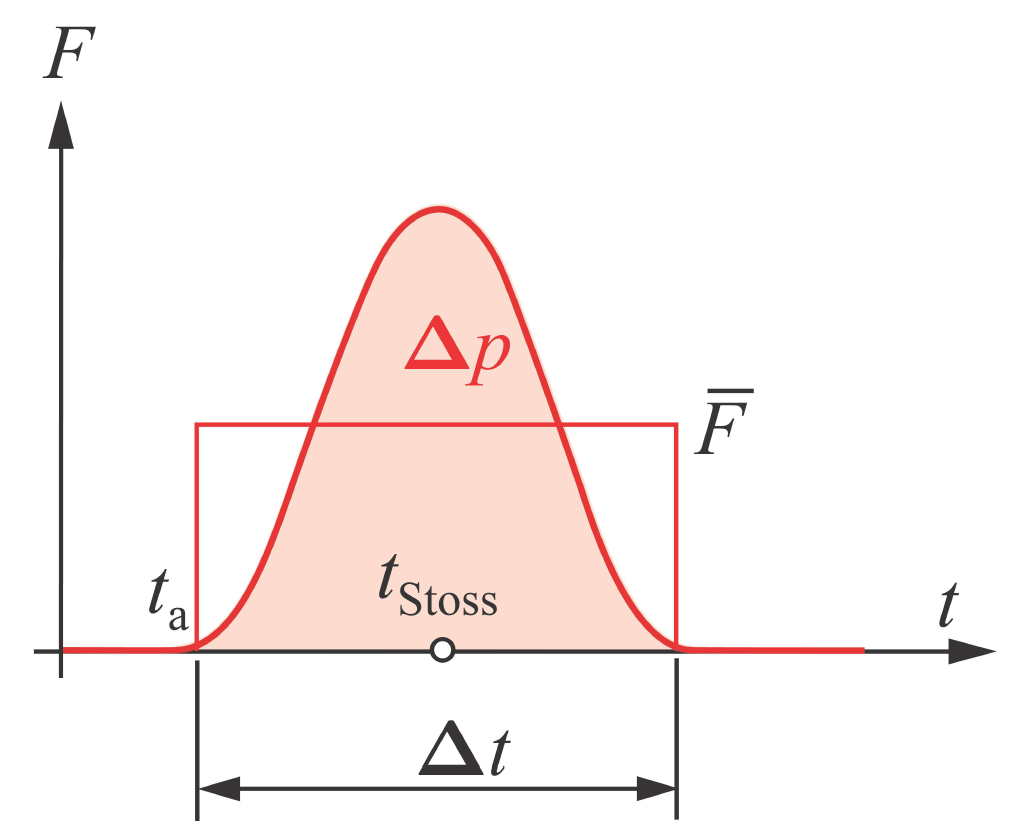
\includegraphics[width=0.8\linewidth]{Bilder/impuls} \\
			\end{minipage}
			
			\begin{tabular}{c l c}
				$F(t)$ & Kraftverlauf & $[F] = \mathrm{N}$ \\
				$\overline{F}$ & mittlere Kraft & $[\overline{F}] = \mathrm{N}$ \\
				$\Delta t$ & Zeitdauer des Kraftstosses & $[\Delta t] = \mathrm{s}$ \\
				$\Delta p$ & Impulsänderung & $[\Delta p] = \mathrm{Ns}$ \\
				$p$ & Impuls vor dem Stoss & $[p] = \mathrm{Ns}$ \\
				$p'$ & Impuls nach dem Stoss & $[p'] = \mathrm{Ns}$ \\
				$\vec{a}$ & Beschleunigung & $[\vec{a}] = \mathrm{\frac{m}{s^2}}$ \\
			\end{tabular}

	\subsection{Impulserhaltungssatz (Impulssatz)}
		In einem \textbf{abgschlossenen System} bleibt der Gesamtimpuls \\
		konstant \\
		abgeschlossenes System: es wirken keine externen Kräfte \\
		
		$$ \boxed{ \vec{p} =  \int \underbrace{  \frac{d \, \vec{p}}{dt} }_{\substack{F_{aussen} = 0}}   \, dt = c = \text{const} }  $$

	\subsection{Stösse}
	
		\begin{tabular}{ll}
			Elastizitätszahl: & $k = \frac{v_2' - v_1'}{v_1 - v_2} = - \frac{v'_{rel}}{v_{rel}} \geq 0$ \\
			\\
			Deformtionsarbeit: & $Q = (E_1 + E_2) - (E_1' + E_2') \geq 0$  \\
			\\
		\end{tabular}

		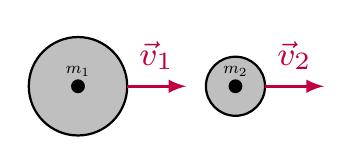
\begin{tikzpicture}
			[
			x=1cm, y=1cm, scale=0.5, font=\footnotesize, >=latex 
			%Voreinstellung für Pfeilspitzen
			]
			%Raster im Hintergrund
			%\draw[step=1, gray, very thin] (0,0) grid (5.5,5.5);
			
			%m1
			\begin{scope}[xshift=0cm, yshift=0cm, rotate=0, scale=1]
				%Kräfte
				\fill[gray!50!white] (0, 0) circle(1.25);
				\draw[thick] (0, 0) circle(1.25);
				\fill[black] (0, 0) circle(5pt) node [midway, above, yshift=2pt, scale=1.5] {$m_1$};
				\draw [-latex, very thick, purple] (1.25,0) -- ++(1.5,0) node[midway, above, scale=1.5] {$\vec{v}_1$};
			\end{scope}		
			
			%m2
			\begin{scope}[xshift=4cm, yshift=0cm, rotate=0, scale=1]
				%Kräfte
				\fill[gray!50!white] (0, 0) circle(0.75);
				\draw[thick] (0, 0) circle(0.75);
				\fill[black] (0, 0) circle(5pt) node [midway, above, yshift=2pt, scale=1.5] {$m_2$};
				\draw [-latex, very thick, purple] (0.75,0) -- ++(1.5,0) node[midway, above, scale=1.5] {$\vec{v}_2$};
			\end{scope}	
		\end{tikzpicture}

		\subsubsection{Gerader, zentraler, total elastischer Stoss}
			Die beiden Stosspartner verformen sich nicht!\\
			$\Rightarrow$ Für die Deformationsarbeit gilt: $Q = 0$ \\
			\boxed{
				\begin{tabular}{ll}
					Impulssatz: &  $p  \overset{!}{=} p'$ \\
					& $m_1 \, v_1 + m_2 \, v_2 \overset{!}{=} m_1 \, v_1' + m_2 \, v_2'$ \\
					\\
					Energiesatz: & $E_{kin} \overset{!}{=} E_{kin}'$ \\
					& $\frac{1}{2} m_1 \, v_1^2 + \frac{1}{2} m_2 \, v_2^2 \overset{!}{=} \frac{1}{2} m_1 \, v_1'^2 + \frac{1}{2} m_2 \, v_2'^2 $ \\
					\\
					& $v_1' = \frac{m_1 - m_2}{m_1 + m_2} \cdot v_1 + \frac{2 \, m}{m_1 + m_2} \cdot v_2$ \\
					\\
					& $v_2' = \frac{2 \, m_1}{m_1 + m_2} \cdot v_1 + \frac{m_2 - m_1}{m_1 + m_2} \cdot v_2$ \\
				\end{tabular}
			}

		\subsubsection{Gerader, zentraler, total inelastischer Stoss}
			Die beiden Stosspartner haften nach dem Stoss aneinander und haben die gleiche Geschwindigkeit. \\
			$\Rightarrow$ Für die Deformationsarbeit gilt: $Q \neq 0$ \\
			\boxed{
				\begin{tabular}{ll}
					Impulssatz: & $p  \overset{!}{=} p'$ \\
					& $m_1 \, v_1 + m_2 \, v_2 \overset{!}{=} (m_1 + m_2) \, v'$ \\
					\\
					Energiesatz: & $E_{kin} \overset{!}{=} E_{kin}'$ \\
					& $\frac{1}{2} m_1 \, v_1^2 + \frac{1}{2} m_2 \, v_2^2 \overset{!}{=} \frac{1}{2} (m_1 + m_2) \, v'^2 + Q$ \\
					\\
					Deformationsarbeit: & $Q = \frac{m_1 \, m_2}{2 (m_1 + m_2)} (v_1 - v_2)^2 =  \frac{1}{2} \mu \cdot v_{rel}^2 $ \\
					\\
					Relativgeschw.: & $v_{rel} := \vert v_1 - v_2  \vert$ \\
					\\
					Reduzierte Masse: & $\mu = \frac{m_1 \, m_2}{m_1 + m_2}$\\
				\end{tabular}
			}

			\begin{tabular}{c l c}
				$k$ & Elastizitätszahl & $[k] = 1$ \\
				$E_1, \,E_2$ & Energien vor Stoss & $[E] = \mathrm{J}$ \\	
				$E_1 ', \, E_2 '$ & Energien nach Stoss & $[E'] = \mathrm{J}$ \\	
				$m_1, \, m_2$ & stossende Massen & $[m] = \mathrm{kg}$ \\
				$v_1, \, v_2$ & Geschwindigkeit vor Stoss & $[v] = \mathrm{\frac{m}{s}}$ \\
				$v_1', \, v_2'$ & Geschwindigkeit nach Stoss & $[v'] = \mathrm{\frac{m}{s}}$ \\
				$Q$ & Deformationsarbeit & $[Q] = \mathrm{J}$ \\
				$v_{rel}$ & Relativgeschwindigkeit &  $[v_{rel}] = \mathrm{\frac{m}{s}}$ \\
				$\mu$ & reduzierte Masse & $[\mu] = \mathrm{kg}$ \\
			\end{tabular}

	\subsection{Rakete}
		\subsubsection{Rakete im Flug}
			$\Rightarrow$ Masse ist hier veränderbar! \qquad $m(t) = m = m_{Start} - \mu \cdot t$ \\
			\\
			Die Rakete verliert an Treibstoff, wodurch die Masse der Rakete abnimmt ($dm < 0$)\\
			\\	
			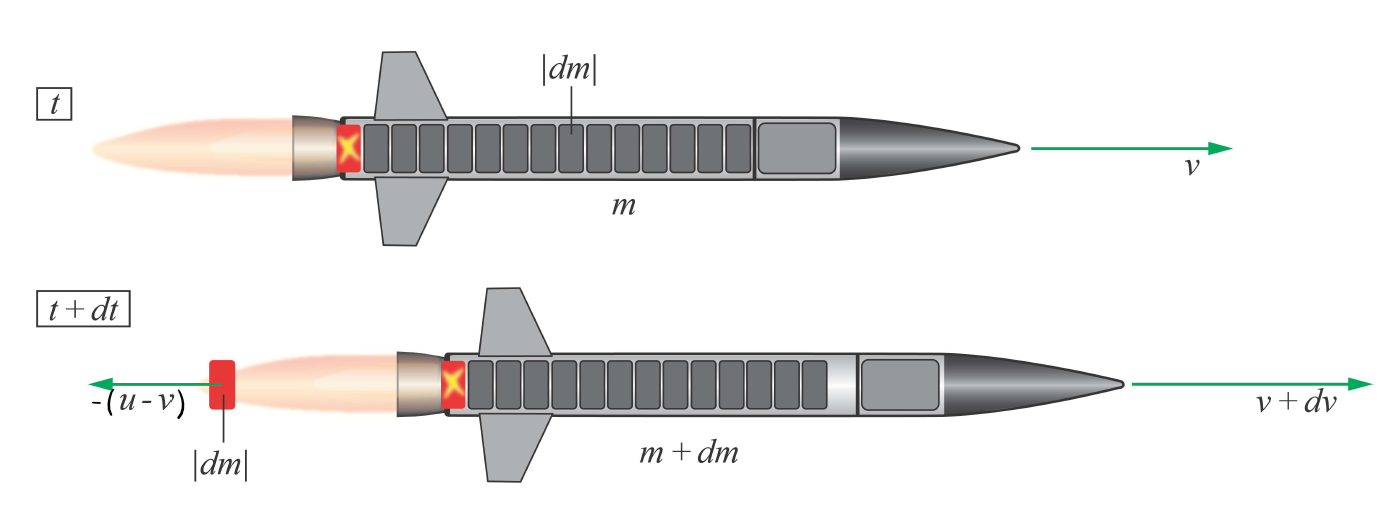
\includegraphics[width=0.73\linewidth]{Bilder/rakete} \\
			\\
			Impulssatz: \quad $ m \cdot v(t) = (m + dm)(v(t) + dv) + dm \,(u-v) $ \qquad $dm < 0$ \\
			\\
			Raketengleichung: $v(t) = - u \cdot \ln(m) + v_0 + u \cdot \ln(m_0) = v_0 + u \cdot \ln(\frac{m_0}{m})$ \\
			\\
			Massenverhältnis: $\frac{Startmasse}{Endmasse}$ \\
			\\
			max. Geschwindigkeitsänderung: $\Delta v = v - v_0 = u \cdot \ln(\frac{m_0}{m})$ \\
			\\
			Schubkraft: $F_{Schub} = \frac{dp}{dt} = - \frac{u \cdot dm}{dt} =  \underbrace{ \frac{dm}{dt} }_{\substack{\mu}} (-u) = \mu \cdot u$ \\ 
			\\
			$\Rightarrow$ Hier wurde noch keine Erdbeschleunigung (Anziehung) berücksichtigt! \\
			\\
			\\
			\begin{tabular}{c l c}
				$u$ &  Strahlgeschwindigkeit der Rakete & $[u] =  \mathrm{\frac{m}{s}}$ \\	
				$m$ & Zeitlich veränderbare Masse $m(t)$ & $[m] = \mathrm{kg}$ \\
				$m_0$ & Masse zum Startzeitpunkt & $[m] = \mathrm{kg}$ \\
				$v_0$ & Startgeschwindigkeit & $[v_0] = \mathrm{\frac{m}{s}}$ \\
				$F_{Schub}$ & Schubkraft der Rakete & $[F_{Schub}] = \mathrm{N}$ \\
				$\mu$ & Treibstoffverbrauch pro Zeit & $[\mu] = \mathrm{\frac{kg}{s}}$
			\end{tabular}

		\subsubsection{Aufstieg der Rakete im Schwerefeld}
			Konstante Erdbeschleunigung g wird berücksichtigt \\
			\\
			Veränderbare Masse: $m(t) = m = m_{Start} - \mu \cdot t$ \\
			\\
			Gesamtkraft: $m(t) \frac{dv}{dt} = m(t) \cdot a = F_{Schub} - F_G = \mu \cdot u - m \cdot g$ \\
			\\
			Beschleunigung: $a(t) = \frac{dv}{dt} = \frac{\mu \cdot u}{m_0 - \mu \cdot t} - g$ \\
			\\
			Raketengleichung: $v(t) = u \cdot \ln( \frac{m_{Start}}{m(t)} ) -  g \cdot t  $ \\
			\\
			Spezifischer Impuls: $T = \frac{m(t)}{\mu} = \frac{u}{g}$ \\
			\\
			\\
			\begin{tabular}{c l c}
				$u$ &  Strahlgeschwindigkeit der Rakete & $[u] =  \mathrm{\frac{m}{s}}$ \\	
				$m$ & Zeitlich veränderbare Masse $m(t)$ & $[m] = \mathrm{kg}$ \\
				$m_0$ & Masse zum Startzeitpunkt & $[m] = \mathrm{kg}$ \\
				$v_0$ & Startgeschwindigkeit & $[v_0] = \mathrm{\frac{m}{s}}$ \\
				$g$ & Erdbeschleuigung & $[g] = \mathrm{\frac{m}{s^2}}$ \\
				$\mu$ & Treibstoffverbrauch pro Zeit & $[\mu] = \mathrm{\frac{kg}{s}}$ \\
				$T$ & spezifischer Impuls (Zeit von konstantem Schub) & $[T] = \mathrm{s}$  \\
			\end{tabular}

	\subsection{Gravitation}
		\subsubsection{Erstes Kepler'sches Gesetz}
			Die Planeten bewegen sich auf Ellipsen, in deren Brennpunkt sich die Sonne befindet. \\
			\\
			\begin{minipage}{0.45\linewidth}
				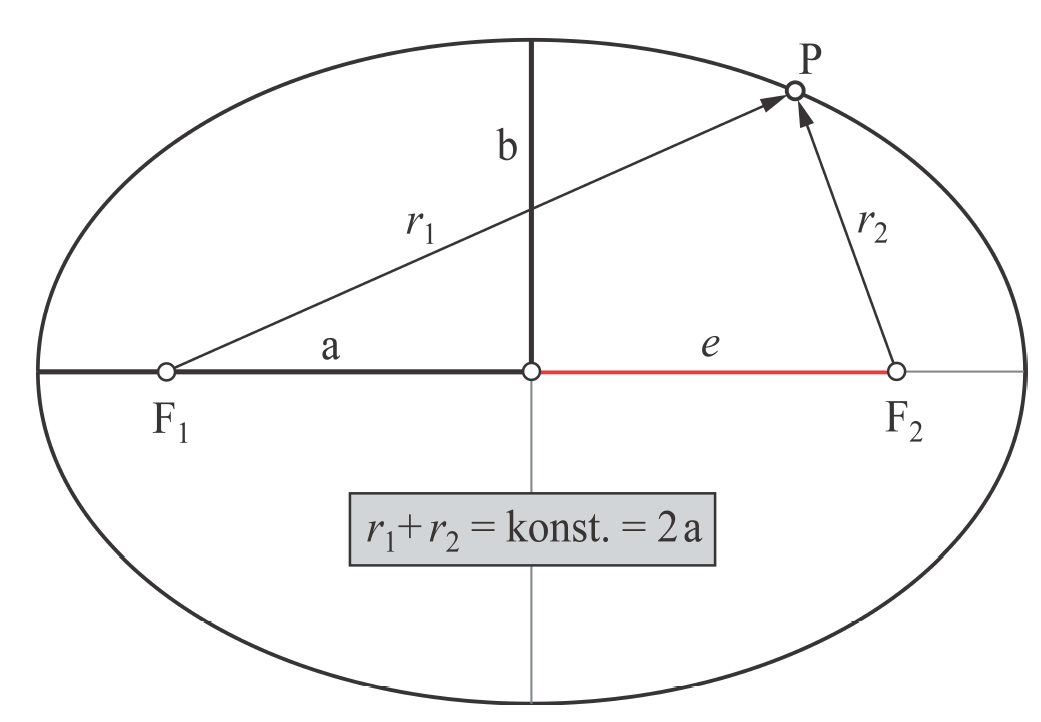
\includegraphics[width=\linewidth]{Bilder/ellipse}
			\end{minipage}
			\hfill
			\begin{minipage}{0.53\linewidth}
				\begin{tabular}{ll}
					$a$ & grosse Halbachse \\
					$b$ & kleine Halbachse \\
					$F_1, F_2$ & Brennpunkte \\
					$e$ & Exzentrizität \\
					$\epsilon$ & num. Exzentrizität $\epsilon = \frac{e}{a} $\\	
					$r_{min}$ & minimaler Radius \\	
					& $r_{min} = a \,(1 - \epsilon)$ \\
					$r_{max}$ & maximaler Radius \\
					& $r_{max} = a \,(1 + \epsilon)$ \\
				\end{tabular}
			\end{minipage}

		\subsubsection{Zweites Kepler'sches Gesetz}
			Der Fahrstrahl der Planeten überstreicht in der gleichen Zeit die gleiche Fläche. \\
			$\Rightarrow$ Bei kleinerem Abstand zur Sonne ist die Geschwindigeit schneller! \\
		
		\subsubsection{Drittes Kepler'sches Gesetz}
			Die Quadrate der Umlaufzeiten verhalten sich wie die Kuben der grossen Halbachsen. \\
			\\
			$a = \big(  \frac{T}{T_{ref}}^{\frac{2}{3}} \cdot a_{ref} \big)$ \qquad $\Leftrightarrow$ \qquad $\big( \frac{a}{a_{ref}}  \big)^3 =  \big( \frac{T}{T_ref}  \big)^2 $ \\
			\\
			Als Referenz wird die Erde verwendet! \\
			\\
			Astronomische Einheit: $a_{ref} = 1 \, \mathrm{AE} = 149.6 \cdot 10^6 \, \mathrm{km}$ \\
			\\
			Referenzzeit: $T_{ref} = 1 \, a = 1 \; \mathrm{Jahr}$ \\
			\\
			\begin{tabular}{c l c}
				$a$ & grosse Halbachse gesuchtet Planet & $[a] = \mathrm{AE}$ \\
				$a_{ref}$ &  grosse Halbachse Erde & $[a_{ref}] = \mathrm{AE}$ \\	
				$T$ & Umlaufzeit Planet & $[T] = \mathrm{Jahre}$ \\
				$T_{ref}$ & Umlaufzeit Erde & $[T] = \mathrm{Jahre}$ \\
			\end{tabular}

		\subsubsection{Gravitationsgesetz}
		
			$$ \boxed{ \text{Gravitationskraft:}  \quad F_G = G \, \frac{m_1 \cdot m_2}{r^2} \quad \text{mit }G = 6.67 \cdot 10^{-11} \mathrm{\frac{m^3}{kg \, s^2}} }$$ 

		\subsubsection{Gravitationswirkung innerhalb einer Kugel}
		
			$$ \boxed{ F_G = G \, \frac{m_{Kern} (r) \, m}{r^2} =  G \, \frac{4 \, \pi \, r^3 \, \rho \, m}{3 \, r^2} = \frac{4 \, pi}{3} \, G \, \rho \, m \, r } $$ \\
		
			\begin{tabular}{c l c}
				$F_G$ & Gravitationskraft & $[F_G] = \mathrm{N}$ \\
				$G$ & Gravitationskonstante & $[G] = \mathrm{\frac{m^3}{kg \, s^2}}$ \\	
				$r$ & Radius (Abstand vom Zentrum) & $[r] = \mathrm{m}$ \\
				$\rho$ & homogene Dichte der Kugel & $[\rho] = \mathrm{\frac{kg}{m^3}}$ \\
				$m$ & Masse vom Massepunkt & $[m] = \mathrm{kg}$ \\
				$m_{Kern}$ & Masse des Kugelkerns & $[m_{Kern}] = \mathrm{kg}$ \\
			\end{tabular}

		\subsubsection{Gravitationswirkung ausserhalb einer Kugel}
		
			$$ \boxed{ F_G = G \, \frac{M \cdot m}{r^2}}  $$ \\
			
			\begin{tabular}{c l c}
				$F_G$ & Gravitationskraft & $[F_G] = \mathrm{N}$ \\
				$G$ & Gravitationskonstante & $[G] = \mathrm{\frac{m^3}{kg \, s^2}}$ \\	
				$r$ & Radius (Abstand vom Zentrum) & $[r] = \mathrm{m}$ \\
				$m$ & Masse vom Massepunkt & $[m] = \mathrm{kg}$ \\
				$M$ & Gesamtmasse der Kugel & $[M] = \mathrm{kg}$ \\
			\end{tabular}

		\subsubsection{Gravitationspotential  $\phi$}
		
			Wenn eine Masse in einem Gravitationsfeld bewegt wird, so wird Arbeit verrrichtet. \\
			\\
			$$ \boxed{ W_{12} = \int \limits_{r_1}^{r_2} \vec{F}_G \bullet d \vec{s}  =  \int \limits_{r_1}^{r_2} G \, \frac{M \cdot m}{r^2} \, dr = G \cdot M \cdot m \big( \frac{1}{r_2} - \frac{1}{r_1}  \big) }  $$  
			
			$$ \boxed{ \text{potentielle Energie:} \quad E_{pot}(r) = -G \, \frac{M \, m}{r} }$$ 
			
			$$ \boxed{ \text{Gravitationspotential:} \quad \phi = \frac{E_{pot}}{m} = - \frac{G \cdot M}{r}}  $$ \\

			\textbf{Im Inneren eines homogenen Zentralkörpers gilt} \\
			
				$$ \boxed{ F_G = \frac{4 \, \pi \cdot G \cdot \rho \cdot m \cdot r}{3} }$$ 
				
				$$ \boxed{ E_{pot} = - \frac{2 \,  \pi \cdot G \cdot \rho \cdot m}{3} \, r^2 + c' } $$
				
				$$ \boxed{ \phi = - \frac{2 \,  \pi \cdot G \cdot \rho}{3} \, r^2 + c = - \frac{G \cdot M(r)}{2 \, r}  + c = - \frac{G \cdot M(r)}{2 \, r} - \frac{G \cdot M}{2 \, R} } $$ \\
				
			\begin{tabular}{c l c}
				$W$ & Arbeit & $[W] = \mathrm{J} $ \\
				$F_G$ & Gravitationskraft & $[F_G] = \mathrm{N}$ \\
				$E_{pot}$ & potentielle Energie & $E_{pot} = \mathrm{J}$ \\
				$G$ & Gravitationskonstante & $[G] = \mathrm{\frac{m^3}{kg \, s^2}}$ \\	
				$r$ & Radius (Abstand vom Zentrum) & $[r] = \mathrm{m}$ \\
				$\rho$ & homogene Dichte der Kugel & $[\rho] = \mathrm{\frac{kg}{m^3}}$ \\
				$m$ & Masse vom Massepunnkt & $[m] = \mathrm{kg}$ \\
				$M$ & Gesamtmasse der Kugel & $[M] = \mathrm{kg}$ \\
				$R$ & Radius der Kugeloberfläche & $[R] = \mathrm{m}$ \\
			\end{tabular}

	\subsection{Bezugssysteme: Inertialsystem}
		Inertialsystem: \textbf{unbeschleuigtes} Bezugssystem \\
		\\
		Wenn die Newton'schen Gesetze im Bezugssystem S gelten, so gelten sie auch im Bezugssystem S', solange dieses nicht beschleunigt ist und nicht rotiert. \\
		$\Rightarrow$ \textbf{In sämtlichen Inertialsystemen sind die mechanischen Gesetze identisch!} \\

		\subsubsection{Galilei-Transformation}
			\begin{minipage}{0.48\linewidth}
				Bezugssystem S' bewegt sich mit konstanter Geschwindigkeit $v_0$: \\
				\\
				\\
				$v_0 = \begin{pmatrix}v_x \\ v_y \\ v_z\end{pmatrix}$
			\end{minipage}
			\hfill
			\begin{minipage}{0.42\linewidth}
				Transformation zwischen \\
				S und S' \\
				\\
				$x = x' + v_x t$ \\
				$y = y' + v_y t$ \\
				$z  = z' + v_z t$ \\
				$t = t'$
			\end{minipage}

	\subsection{Beschleunigte Bezugssysteme}
		In beschleunigten Bezugssystemen müssen \textbf{Trägheitskräfte} berücksichtigt werden!

		\subsubsection{Translatorisch beschleunigtes Bezugssystem}
			Beispiel: Zug beschleunigt auf gerader Schiene \\
			\\
			Für einen Beobachter \textbf{im beschleunigten System} S' wirkt \\
			eine Trägheitskraft: 
			
			$$ \boxed{ \text{Gesamtkraft:} \quad \vec{F}' = \vec{F} - m \cdot \vec{a}_0 = \vec{F} + \vec{F}_{Tr"agheit} }$$ \\
			
			\begin{tabular}{c l c}
				$\vec{F}'$ & Gesamte im System wirkende Kraft & $[\vec{F}'] = \mathrm{N}$ \\
				$\vec{F}$ & Statisch wirkende Kräfte & $[\vec{F}] = \mathrm{N}$ \\
				$\vec{F}_{Tr"agheit}$ & Trägheitskraft & $[\vec{F}_{Tr"agheit}] = \mathrm{N}$ \\
				$m$ & Masse im System & $[m] = \mathrm{kg}$ \\
				$\vec{a}_0$ & Beschleunigung des Systems & $[\vec{a}_0] = \mathrm{\frac{m}{s^2}}$ \\
			\end{tabular}

		\subsubsection{Gleichförmig rotierendes Bezugssystem (Scheinkräfte)}

			\textbf{Fest verbundene Masse} $\Rightarrow$ \textbf{Scheinkraft: Zentrifugalkraft} \\
				\\
				\begin{minipage}{0.48\linewidth}
					$$ \boxed{ \vec{F}_z = - m \, \vec{a}_z = - m \cdot \omega^2 \cdot \vec{r} }$$ 
					
					$$ \boxed{ \vec{F}_{Zentrifugal}  \overset{!}{=} - \vec{F}_{Zentripetal} }$$ 
				\end{minipage}
				\hfill
				\begin{minipage}{0.48\linewidth}
					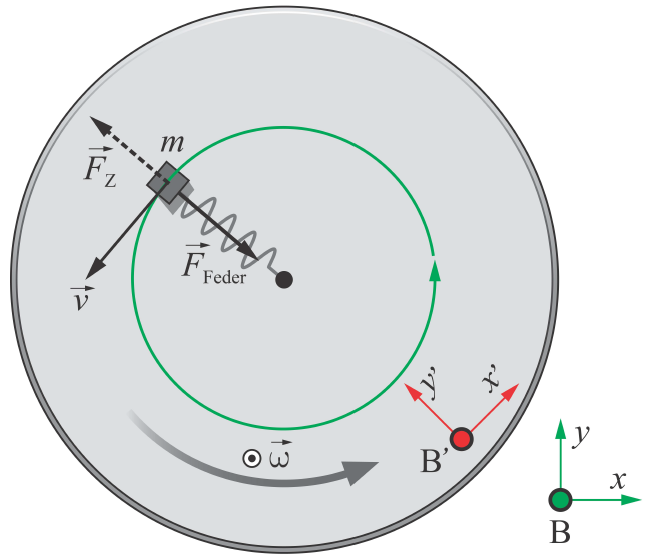
\includegraphics[width=0.75\linewidth]{Bilder/zentrifugalkraft} \\
				\end{minipage}
				\\
				\begin{tabular}{c l c}
					$\vec{F}_z$ & Zentrifugalkraft (Trägheitskraft; Scheinkraft) & $[\vec{F}_z] = \mathrm{N}$ \\
					$m$ & Masse im System & $[m] = \mathrm{kg}$ \\
					$\vec{a}_z$ & Beschleunigung des Systems ($a_{radial}$) & $[\vec{a}_z] = \mathrm{\frac{m}{s^2}}$ \\
					$\omega$ & Winkelgeschwindigkeit & $[\omega] = \mathrm{\frac{rad}{s}}$ \\
					$\vec{r}$ & Radius des Systems (nach innen zeigend) & $[\vec{r}] = \mathrm{m}$ \\ 
					\\
					\\
				\end{tabular}

			\textbf{lose Masse} $\Rightarrow$ \textbf{Scheinkraft: Corioliskraft} \\	
				\\
				\\
				\begin{minipage}{0.48\linewidth}
					$$ \boxed{\vec{F}_c = - m \cdot \vec{a}_c = - m \cdot 2 \, (\vec{\omega} \times \vec{v}_R)} $$ 
				\end{minipage}
				\hfill
				\begin{minipage}{0.48\linewidth}
					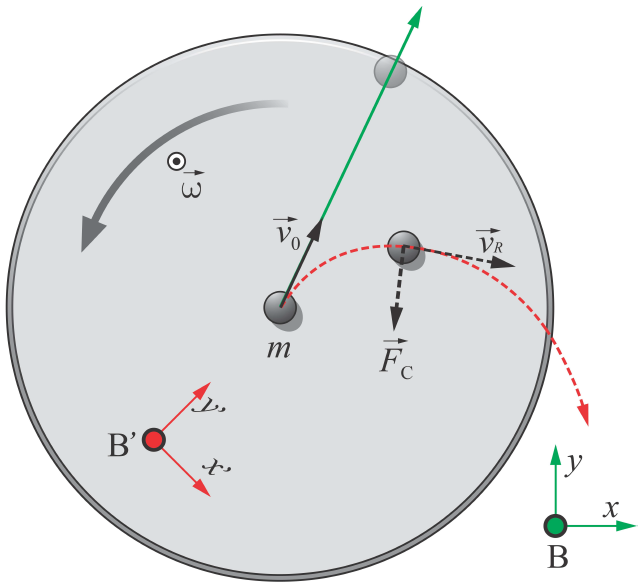
\includegraphics[width=0.75\linewidth]{Bilder/corioliskraft} \\
				\end{minipage}
				\\
				\begin{tabular}{c l c}
					$\vec{F}_c$ & Corioliskraft (Trägheitskraft; Scheinkraft) & $[\vec{F}_c] = \mathrm{N}$ \\
					$m$ & Masse im System & $[m] = \mathrm{kg}$ \\
					$\vec{a}_c$ & Coriolisbeschleunigung & $[\vec{a}_c] = \mathrm{\frac{m}{s^2}}$ \\
					$\omega$ & Winkelgeschwindigkeit & $[\omega] = \mathrm{\frac{rad}{s}}$ \\
					$\vec{v}_R$ & Relativgeschwindigkeit & $[\vec{v}_R] = \mathrm{\frac{m}{s}}$ \\ 
				\end{tabular}

		\subsubsection{D'Alembert'sches Prinzip}
			Wird ein Körper in einem mitbewegten Koordinatensystem \\
			betrachtet, so bleibt er in Ruhe: \quad $\vec{v}_R = 0$ und $\vec{a}_R = 0$ \\
			
			$$ \boxed{ \vec{F} + \underbrace{ \vec{F}_z + \vec{F}_c }_{\substack{\text{Scheinkräfte}}} = \vec{0} }$$ 
			
			$\Rightarrow$ Statisches Gleichgewichtsproblem

	\subsection{Rotation starrer Körper}
	
		\begin{tabular}{ll}
			Rotation: & Drehung um feste Achse \\
			Kreisel: & Drehung um starren Punkt \\
			Kreiselbewegung & Drehung eines völlig freien, \\
			&  starren Körpers um seinen Schwerpunkt \\
		\end{tabular}

		\subsubsection{Dynamisches Grundgesetz der Rotation}
			Es ist \textbf{nur die tangentiale Komponente} der Kraft \\
			(des Drehmoments) eines rotierenden Körpers relevant! \\
				
			$$dM_t = r \cdot dF_t = r \cdot dm \cdot a_t = dm \cdot r^2 \cdot \alpha$$ \\
			
			$$ \boxed{ M = \int dM = \int r^2 \, \alpha \cdot dm = \alpha  \underbrace{  \int r^2 \cdot dm }_{\substack{J_{Scheibe} = m \cdot r^2}} }$$ \
			
			$$ \boxed{ \Rightarrow \; M = J \cdot \alpha} $$ \\
				
			\begin{tabular}{c l c}
				$dM_t$ & kleine Tan.-Komponente des Drehmoments & $[dM_t] = \mathrm{Nm}$ \\
				$M$ & (gesamtes) Drehmoment & $[M] = \mathrm{Nm}$ \\
				$dF_t$ & kleine Tangentialkomponente der Kraft & $[dF_t] = \mathrm{N}$ \\
				$r$ & Abstand Drehachse zu Massepunkt (Rand) & $[r] = \mathrm{m}$ \\
				$dm$ & kleines Massestück des Körpers & $dm = \mathrm{kg}$ \\
				$a_t$ & Tangentialbeschleunigung ($a_t = r \cdot \alpha$) & $[a_t] = \mathrm{\frac{m}{s^2}}$ \\
				$\alpha$ & Winkelbescheunigung & $[\alpha] = \mathrm{\frac{rad}{s^2}}$ \\
				$J$ & (Massen-) Trägheitsmoment & $[J] = \mathrm{kg \, m^2}$ \\
			\end{tabular}

		\subsubsection{Massenträgheitsmomente}
		
			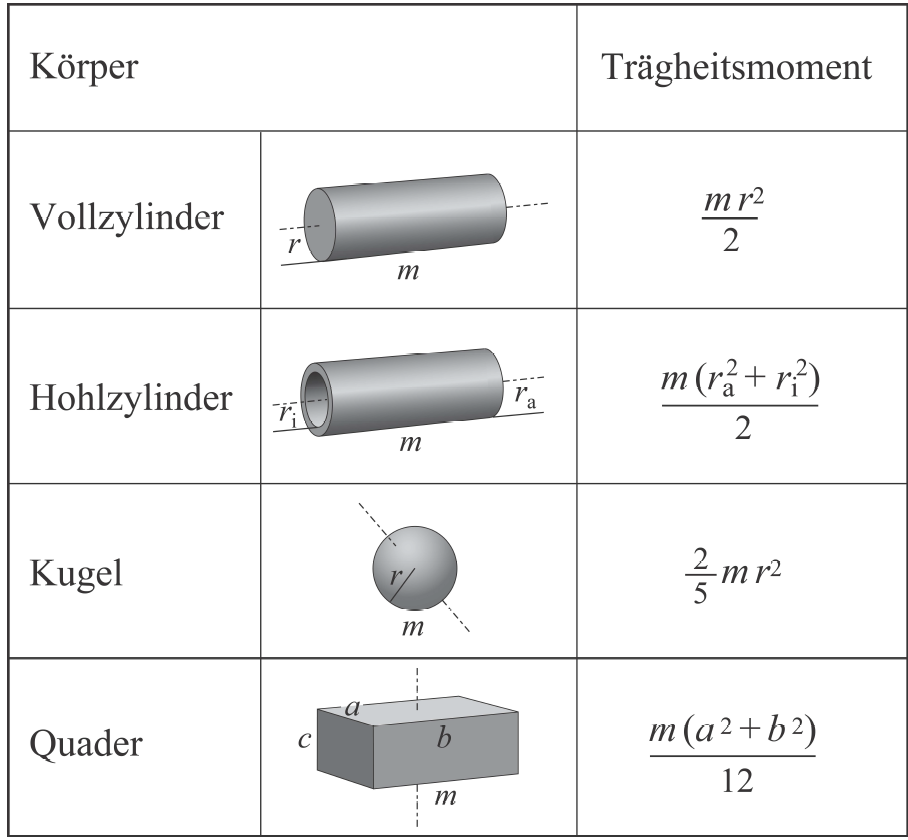
\includegraphics[width=0.8\linewidth]{Bilder/massentraegheitsmomente}

	\subsection{Trägheitsellipsoid}
		Trägheitsradius $r_0$: als ob ganze Masse eines Körpers nur einen \\
		Radius hätte \\
		\\
		\begin{minipage}{0.48\linewidth}
			$$ \boxed{ r_0 = \sqrt{\frac{J}{m}}} $$
		\end{minipage}
		\hfill
		\begin{minipage}{0.48\linewidth}
			$$ \boxed{s_0 = \frac{1}{r_0} }$$
		\end{minipage}
		
		\begin{tabular}{c l c}
			$r_0$ & Trägheitsradius & $[r_0] = \mathrm{m}$ \\
			$m$ & Masse des Körpers & $[m] = \mathrm{kg}$ \\
			$J$ & (Massen-) Trägheitsmoment & $[J] = \mathrm{kg \, m^2}$ \\
			$s_0$ & reziproker Trägheitsradius & $[s_0] = \mathrm{m}$ \\
			\\
		\end{tabular}
		
		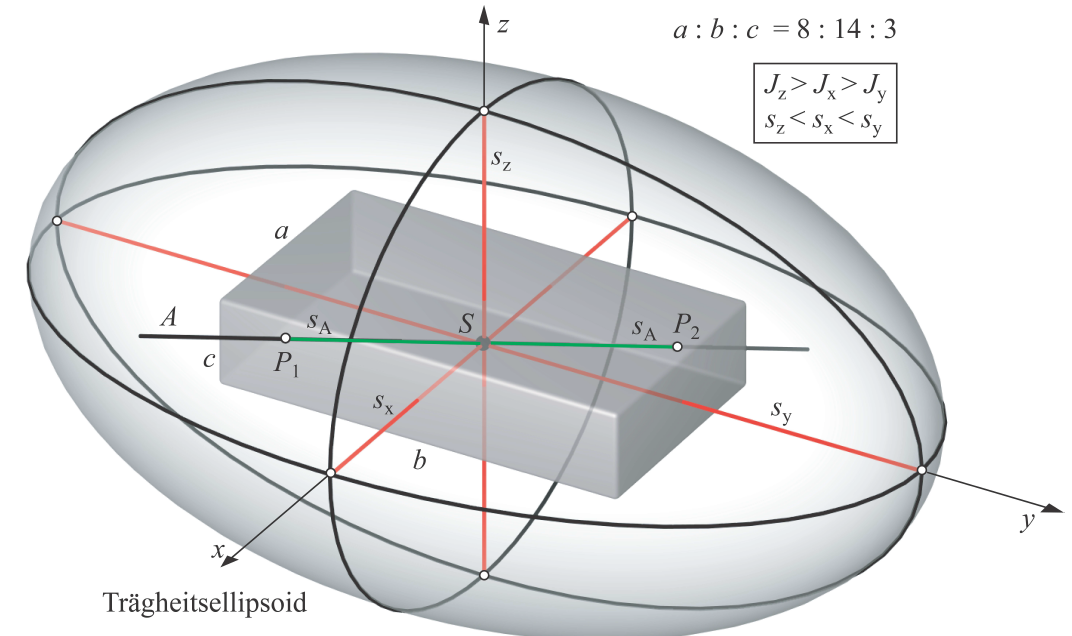
\includegraphics[width=0.8\linewidth]{Bilder/traegheits_ellipsoid} \\	
		\\
		\textcolor{red}{Hauptträgheits-Achsen} (entsprechen immer Symmetrie-Achsen, falls vorhanden) \\
		\textcolor{green}{beliebige Achse $J_A$} \quad $J_A = J_x \cdot \cos^2(\alpha) + J_y \cdot \cos^2(\beta) + J_z \cdot \cos^2(\gamma)$

	\subsection{Satz von Steiner}
		Beschreibt, wie man das Trägheitsmoment $J$ berechnet, wenn die Drehachse nicht durch den Schwerpunkt des rotierenden Körpers geht, sonden \textbf{parallel} dazu verläuft. \\
		
		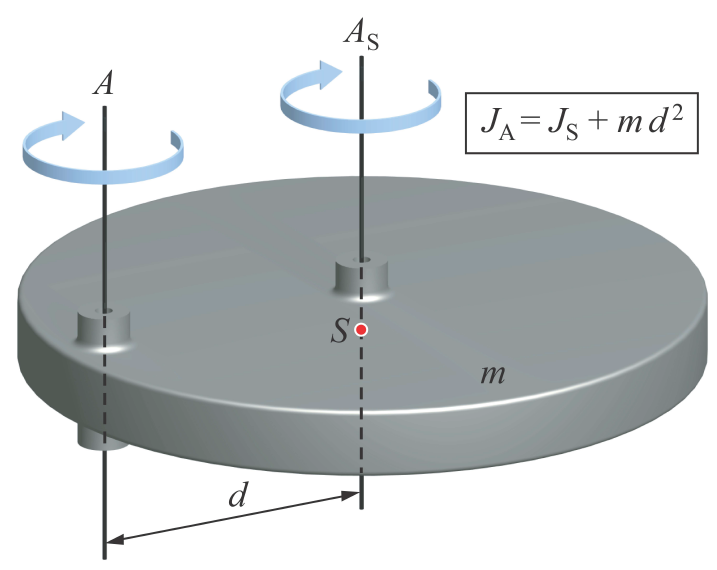
\includegraphics[width=0.6\linewidth]{Bilder/steiner} \\	
		\\
		\begin{tabular}{c l c}
			$J_S$ & Trägheitsmoment (Rot. um Schwerp.)  & $[J_S] = \mathrm{kg \, m^2}$ \\
			$J_A$ & Trägheitsmoment (Rot. um bel. Punkt)  & $[J_A] = \mathrm{kg \, m^2}$ \\
			$m$ & Masse des Körpers & $[m] = \mathrm{kg}$ \\
			$d$ & Abstand zum Schwerpunkt & $[d] = \mathrm{m}$ \\
		\end{tabular}

	\subsection{Arbeit und Leistung (Rotation)}
		$dW = \vec{F} \bullet d\vec{s} = F_t \cdot ds = F_t \cdot r \cdot d \phi = M \cdot d \phi $ \\
		\\
		$P = \frac{dW}{dt} = M \frac{d \phi}{dt} = M \cdot \omega$ \\
		\\
		\begin{tabular}{c l c}
			$F_t$ & \textbf{Tantentialer} Kraftanteil der Rotation & $[F_t] = N$ \\
			$d \phi$ & zurückgelegter Kreiswinkel & $[d \phi] = rad$ \\	
			$P$ & Leistung  & $[P] = W$ \\
			$W$ & Energie  & $[W] = J$ \\
			$\omega$ & Winkelgeschwindigkeit & $[\omega] = \frac{rad}{s}$ \\
			$M$ & Drehmoment & $[M] = Nm$ \\
		\end{tabular}

	\subsection{Rotationsenergie}
		\textbf{Folgendes gilt nur für die Rotation um den Schwerpunkt eines Körpers!} \\
		
		Die totale kinetische Energie ist die Summe aller kinetischer Energien eines Körpers \\
		
		$$ \boxed{ E_{kin} = \int \frac{1}{2} \, v^2 \, dm  = E_{trans} + E_{rot} } $$ 
		
		\begin{minipage}{0.48\linewidth}
			$$ \boxed{ E_{trans} = \frac{1}{2} \, m \cdot v_s^2 } $$ 
		\end{minipage}
		\hfill
		\begin{minipage}{0.48\linewidth}
			$$ \boxed{ E_{rot} = \frac{1}{2} \, J_s \cdot \omega^2 } $$ 
		\end{minipage}

		\begin{tabular}{c l c}
			$E_{trans}$ & Translationsenergie des Schwerpunkts & $[E_{trans}] = \mathrm{J}$ \\
			$m$ & Masse des Körpers & $[m] = \mathrm{kg}$ \\
			$v_s$ & Geschwindigkeit des Schwerpunkts & $[v_s] = \mathrm{\frac{m}{s}}$ \\
			$E_{rot}$ & Rotationsenergie & $[E_{rot}] = \mathrm{J}$ \\
			$J_S$ & Trägheitsmoment (Rot. um Schwerp.)  & $[J_S] = \mathrm{kg \, m^2}$ \\
			$\omega$ & Winkelgeschwindigkeit & $[\omega] = \mathrm{\frac{rad}{s}}$ \\
		\end{tabular}
	 
	\subsection{Drehimpuls $\vec{L}$ / Impulserhaltung (Rotation)}
		\begin{minipage}{0.42\linewidth}
			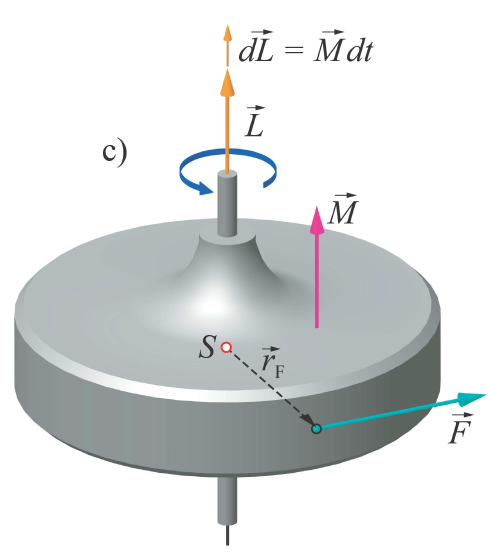
\includegraphics[width=\linewidth]{Bilder/drehimpuls} \\
			\\
		\end{minipage}
		\hfill
		\begin{minipage}{0.56\linewidth}
			$$ \boxed{ \vec{L} = \int d \vec{L} = \int \vec{r} \times \vec{v} \cdot dm = \vec{r} \times \vec{p} }$$ \\
		\end{minipage}

		\begin{tabular}{c l c}
			$\vec{L}$ & Drehimpuls & $[\vec{L}] = \mathrm{\frac{kg \, m^2}{s}}$ \\
			$\vec{r}$ & Abstand Massepunkt zu Rot-Achse & $[\vec{r}] = \mathrm{m}$ \\
			$\vec{v}$ & Rotationsgeschwindigkeit & $[\vec{v}] = \mathrm{\frac{m}{s}}$ \\
			$dm$ & kleines Masse-Stück & $[dm] = \mathrm{kg}$ \\
			$\vec{p}$ & Impuls & $[\vec{p}] = \mathrm{\frac{kg \, m}{s}}$ \\
		\end{tabular}

		\subsubsection{Drehmoment $\vec{M}$ vs. Drehimpuls $\vec{L}$}
			$$ \boxed{ \vec{M} = \vec{r} \times \vec{F} = \frac{d}{dt} (\vec{r} \times \vec{p}) =  \frac{d}{dt} \vec{L} = \dot{\vec{L}} }$$ \\
			
			\textbf{In einem abgschlossenen System ($\vec{M} = 0$) bleibt der \\
			Gesamtdrehimpuls erhalten} \\
			$\Rightarrow \vec{L} = \text{const}$ \\
			\\
			\boxed{
				\begin{tabular}{ll}
					Impulserhaltung: &  $L  \overset{!}{=} L'$ \\
					& $J_1 \cdot \omega + J_2 \cdot \omega \overset{!}{=} J_1 \cdot \omega_1' + J_2 \cdot \omega_2'$ \\
					\\
					Energiesatz: & $E_{rot} \overset{!}{=} E_{rot}' + Q$ \\
					& $\frac{1}{2} J_1 \cdot \omega_1^2 + \frac{1}{2} J_2 \cdot \omega_2^2 \overset{!}{=} \frac{1}{2} J_1 \cdot \omega_1'^2 + \frac{1}{2} J_2 \cdot \omega_2'^2 + Q $ \\
				\end{tabular}
			}
			\\
			\\
			\begin{tabular}{c l c}
				$\vec{M}$ & Drehmoment & $[\vec{M}] = \mathrm{Nm}$ \\
				$\vec{r}$ & Abstand Massepunkt zu Rot-Achse & $[\vec{r}] = \mathrm{m}$ \\
				$\vec{F}$ & Kraft, welche Drehmoment bewirkt & $[\vec{F}] = \mathrm{N}$ \\
				$\vec{p}$ & Impuls & $[\vec{p}] = \mathrm{\frac{kg \, m}{s}}$ \\
				$\vec{L}$ & Drehimpuls & $[\vec{L}] = \mathrm{\frac{kg \, m^2}{s}}$ \\
				$J$  & Massenträgheitsmoment & $[J] = \mathrm{kg \, m^2}$ \\
				$\omega$ & Winkelgeschwindigkeit & $[\omega] = \mathrm{\frac{1}{s}}$ \\
				$Q$ & Deformationsarbeit & $[Q] = \mathrm{J}$ \\
			\end{tabular}

		\subsubsection{Drehimpuls $\vec{L}$ vs. Winkelgeschwindigkeit $\omega$}

		$$ \boxed{ L = \int dL = \int r^2 \, \omega \, dm = \omega \int r^2 \, dm = J \, \omega }$$ \\
		
			\begin{tabular}{c l c}
				$L$ & Drehimpuls & $[L] = \mathrm{\frac{kg \, m^2}{s}}$ \\
				$r$ & Abstand Massepunkt zu Rot-Achse & $[r] = \mathrm{m}$ \\
				$dm$ & kleines Masse-Stück & $[dm] = \mathrm{kg}$ \\
				$\omega$ & Winkelgeschwindigkeit & $[\omega] = \mathrm{\frac{rad}{s}}$ \\
				$J$ & (Massen-) Trägheitsmoment (hier Tensor) & $[J] = \mathrm{kg \, m^2}$ \\
			\end{tabular}

	\subsection{Rotation vs. Translation}
	
		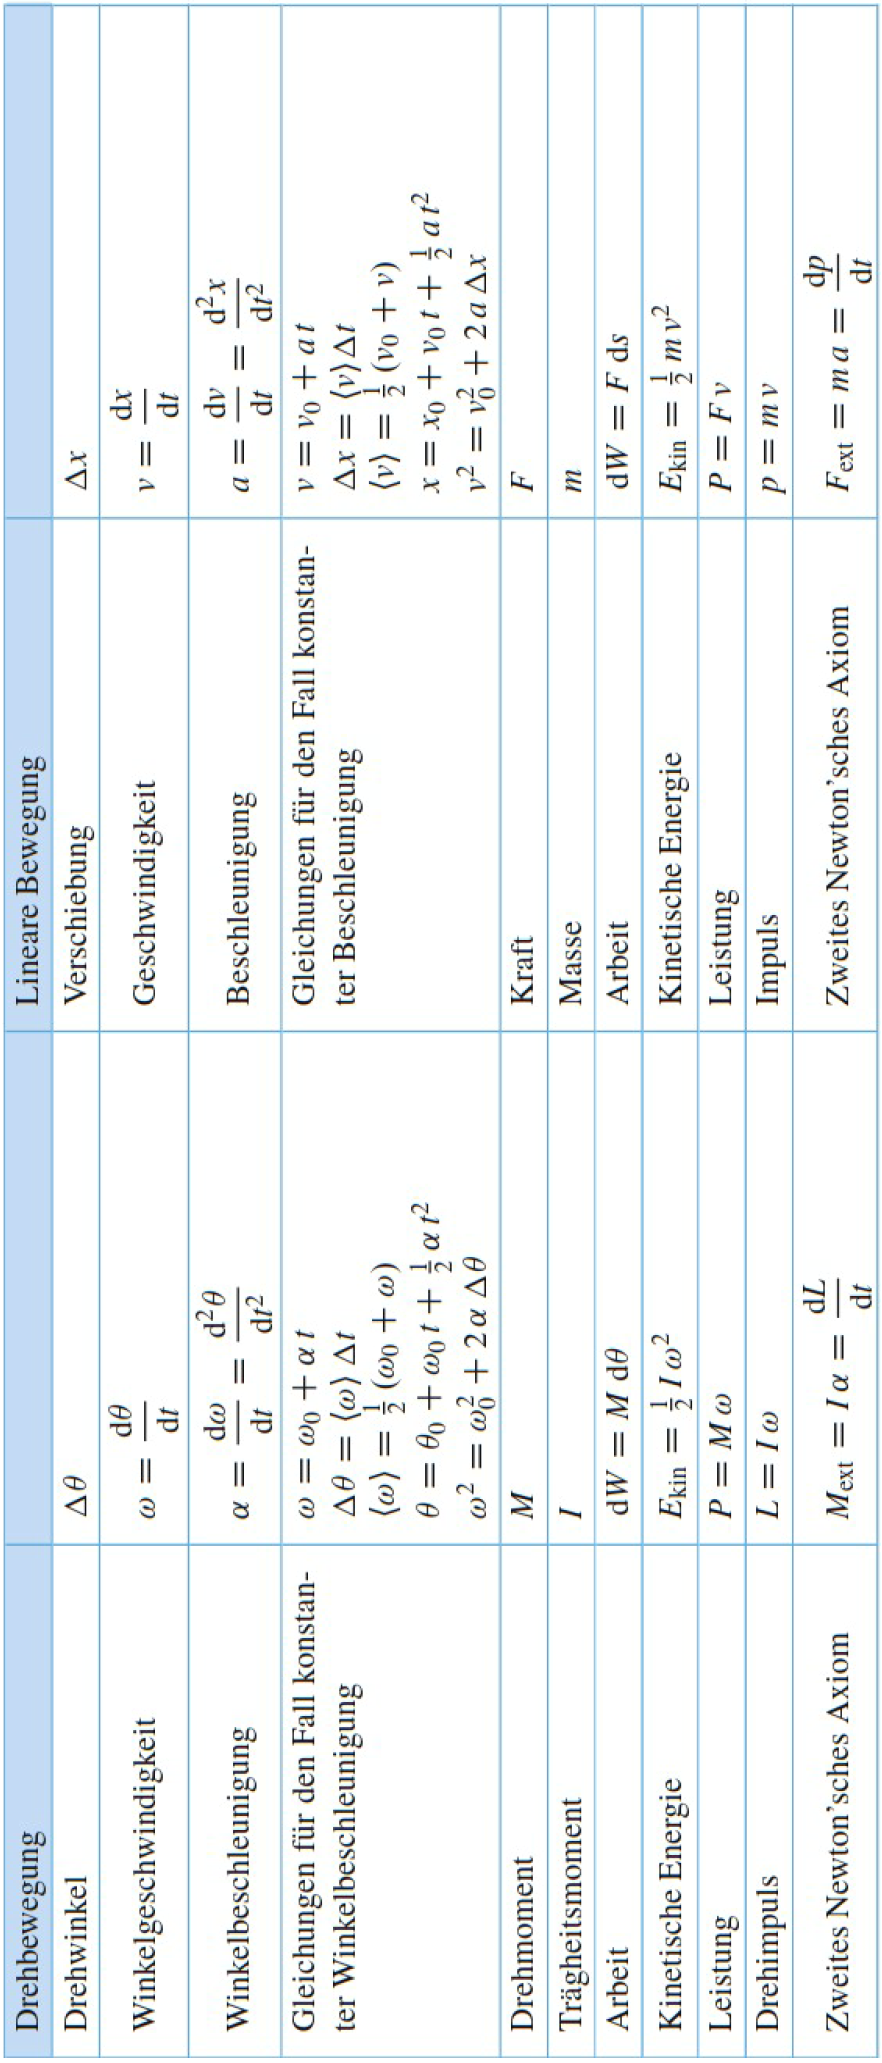
\includegraphics[width=0.85\linewidth]{Bilder/rotation_translation}
		